\documentclass[a4paper,10pt]{article}

% \usepackage{natbib}
\usepackage{amsthm}
\usepackage{amsfonts}
\usepackage{amssymb}
\usepackage{amsmath}
\usepackage{latexsym}
\usepackage{graphicx}
\usepackage{blindtext}
\usepackage{float}

\usepackage{doc}

\newtheorem*{theorem}{Theorem}
\theoremstyle{definition}
\newtheorem*{definition}{Definition}

\hoffset -1in \topmargin 0mm \voffset 0mm \headheight 0mm
\headsep0mm
\oddsidemargin  20mm     %   Left margin on odd-numbered pages.
\evensidemargin 20mm     %   Left margin on even-numbered pages.
\textwidth   170mm       %   Width of text line.
\textheight  252mm

\makeatletter
\renewcommand\@openbib@code{%
     \advance\leftmargin  \z@ %\bibindent
      \itemindent \z@
     % Move bibitems close together
     \parsep -0.8ex
     }
\makeatother

\makeatletter
\renewcommand\section{\@startsection {section}{1}{\z@}%
                                   {-3.5ex \@plus -1ex \@minus -.2ex}%
                                   {1.5ex \@plus.2ex}%
                                   {\large\bfseries}}
\makeatother

\makeatletter
\renewcommand\subsection{\@startsection {subsection}{1}{\z@}%
                                   {-3.5ex \@plus -1ex \@minus -.2ex}%
                                   {1.5ex \@plus.2ex}%
                                   {\normalsize\bfseries}}
\makeatother

\makeatletter
	\setlength{\abovecaptionskip}{3pt}   % 0.25cm 
	\setlength{\belowcaptionskip}{3pt}   % 0.25cm 
\makeatother

\begin{document}
\pagestyle{empty}

\begin{center}
{\bf \Large Drones in agriculture 4.0}
\end{center}

\smallskip
\begin{center}
{\large Jan Fiala}
\end{center}

\smallskip
\begin{center}
Faculty of Mechanical Engineering, Brno University of Technology\\
Institute of Automation and Computer Science\\
Technicka 2896/2, Brno 616 69, Czech Republic\\
217141@vutbr.cz\\
\end{center}

\bigskip
\noindent Abstract: \textit{This seminar paper deals with remarkable development in recent decades of agriculture 4.0. Especially about agriculture drones, which significantly improve and innovate current farming activities with increased efficiency and efficacy. }


\vspace*{10pt} \noindent Keywords: \textit{Drones, UAV, Precision agriculture, Agriculture 4.0}

\bigskip
\section{Introduction}
\label{sec:1}

Agriculture 4.0 represents the fourth agriculture revolution that uses digital technologies and moves toward a more efficient, smart, environmentally responsible agriculture sector. Farming technologies have emerged to enhance sustainability and discover more effective farm methods, including digitalization and automation processes in business and our daily lives, including Artificial Intelligence (AI) and robots (see Fig.~\ref{fig:1}). 

Drones, also called Unmanned Aerial Vehicles (UAV), have witnessed a remarkable development in recent decades. In agriculture, they have changed farming practices by offering farmers substantial cost savings, increased operational efficiency, and better profitability. We can divide them into groups with different benefits that they provides.\cite{JAVAID2022150,REJEB2022107017}

\begin{figure}[h]
\begin{center}
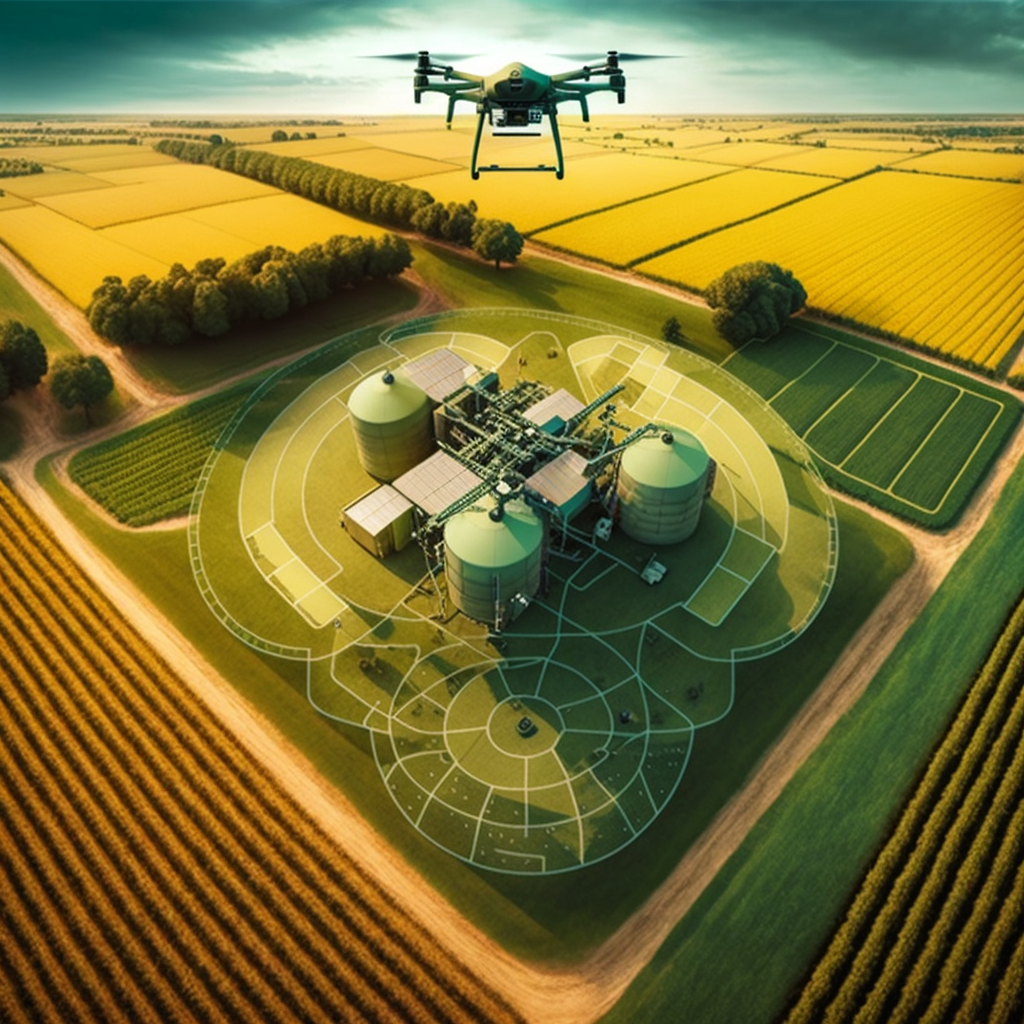
\includegraphics[scale=0.27]{images/Fialin_agriculture_4.0_drone_scanning_0123ab8e-99cf-4ebe-9375-09f6d7ebec64.png}
\caption{Agriculture 4.0 theme generated by AI}
\cite{droneAI}
\label{fig:1}
\end{center}
\end{figure}

\section{Main benefits of drones in agriculture}
\label{sec:2}
As a multidisciplinary and multipurpose technology in agriculture, drones have been investigated from various perspectives. They can be used for different applications, contributing to precision agriculture, with their navigational and sensing capabilities. Precision agriculture comprises a set of technologies that combines sensors, information systems, enhanced machinery, and informed management to optimize production by accounting for variability and uncertainties within agricultural systems. \cite{REJEB2022107017}

\subsection{Drone mapping}
\label{subsec:1}
Accurate soil data, which can be collected with agricultural sensors spaced at the half-variogram range, is crucial information for precision agriculture. Drones offer a unique advantage over other existing methods to sample data from soil sensors because of the high density of sensors required to gather spatially granular data to capture soil variability. 

Built-in sensors will come with ground sensors, so soil moisture, temperature, humidity, and other vital information are updated for the farmer’s reference.  Possible attachments are pictured in Fig.~\ref{fig:2}. \cite{rs12030514,GOODRICH2023107591}


\begin{figure}[h]
\begin{center}
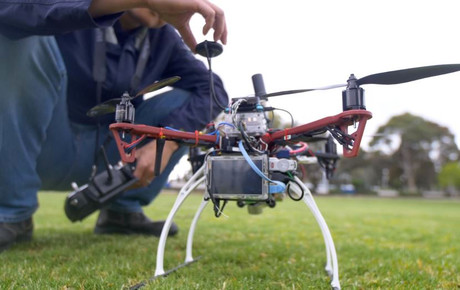
\includegraphics[scale=0.9]{images/Soil-Mapping-1-HR-.jpg}
\caption{The Autonomous Drones for Soil Moisture Mapping project}
\cite{drone_facilitates}
\label{fig:2}
\end{center}
\end{figure}

\subsection{Classification and scouting of crops}
\label{subsec:2}
Maintaining land, crops, stables, and livestock can take a lot of time. Other big issues are limited spotting potential and scan distance on foot. Drone technology provides more in-depth results in real-time. With images collected from a farming drone, farmers can get high-definition photos, videos, and data within minutes. With the benefits of a bird's eye view, it’s easier to spot crop issues or potential safety problems and act quickly, even on hectares of fields in a single flight. For this observation, they use thermal and multispectral cameras, mounted to the downside of the quadcopter (see Fig.~\ref{fig:3}), to record the reflectance of the vegetation.
\cite{drones4030041, SUBRAMANIAM2021}

\begin{figure}[h]
\begin{center}
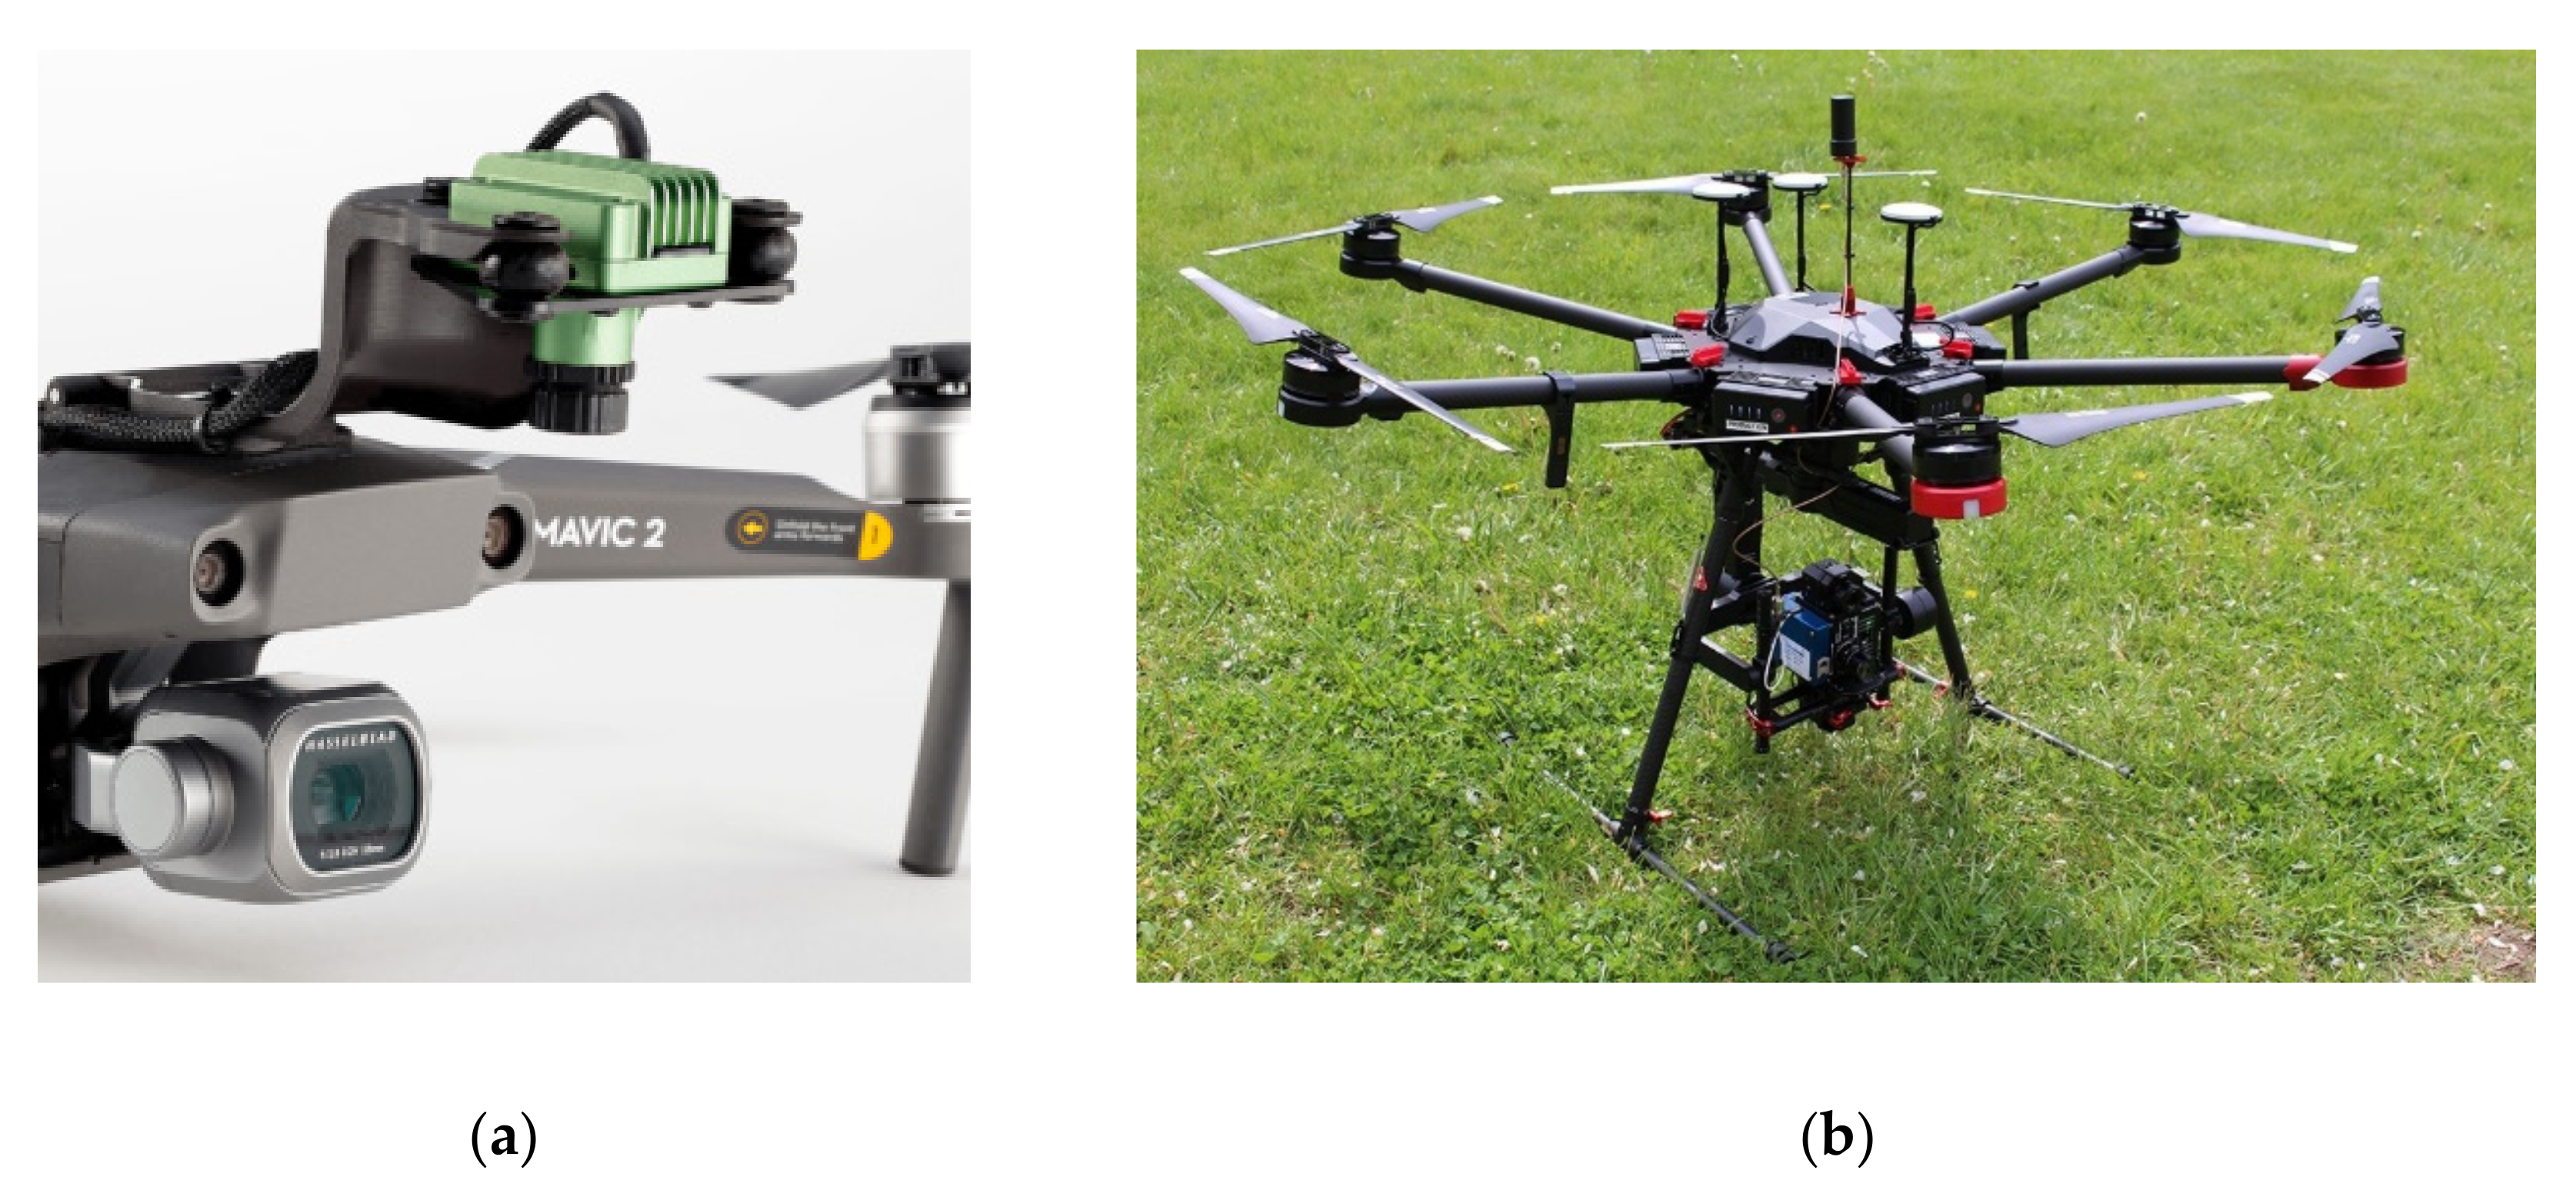
\includegraphics[scale=0.1]{images/drones-04-00041-g003.png}
\caption{Possible positions of sensors and cameras on drone}\cite{drones4030041}
\label{fig:3}
\end{center}
\end{figure}

\subsection{Aerial spraying, seeding, and watering}
\label{subsec:3}
Aerial distribution is a function of drones where they fly over a specific terrain equipped with a smart dispersal mechanism to plant-specific load to desired areas. Aerial spraying drones are tank-carrying UAVs that spray crops with fertilizers or pesticides. Unlike a traditional tractor, drones can spray crops more precisely. Because they can be programmed to spray an even amount of liquid in all necessary sections.

Seeding is another activity that drones can perform If surveying was done right, the drone will have data on soil hardness and adjust the pressure for firing the seed pods (Fig.~\ref{fig:4}), so the soil is penetrated effectively. 

One of the biggest advantages of using a drone for watering is its ability to track water needs. Using infrared technology, an aerial vehicle like this will be able to determine water absorption levels. This means that the user will have access to data on which areas are getting too little, the right amount, or too much water. 
\cite{doi:10.1080/00380768.2020.1738899,agriculture_spreading, SUBRAMANIAM2021}

\begin{figure}[h]
\begin{center}
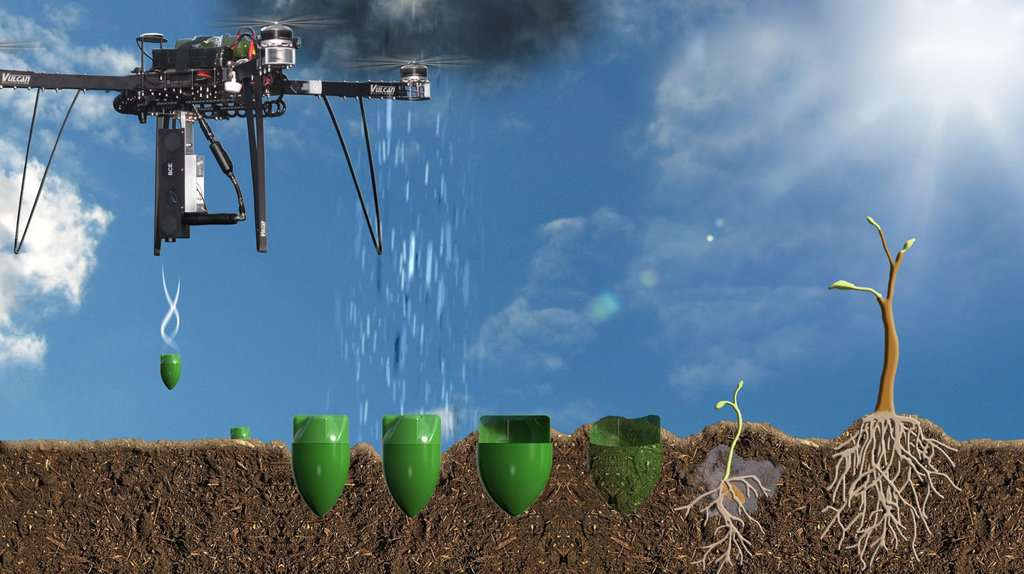
\includegraphics[scale=0.3]{images/Biodegradable-seedpods.jpg}
\caption{Advanced drone seeding system with fertilizer capsule}\cite{doi:10.1080/00380768.2020.1738899}
\label{fig:4}
\end{center}
\end{figure}

\subsection{Animals and disease detection}
\label{subsec:4}
 The proliferation of relatively affordable off-the-shelf drones offers great opportunities for wildlife monitoring. Similarly, the recent reduction in the cost of thermal infrared cameras also offers new promise in this field, as they have the advantage over conventional RGB cameras of being able to distinguish animals based on their body heat (Fig.~\ref{fig:5}) and being able to detect animals at night.
\cite{animals_drone}

\begin{figure}[h]
\begin{center}
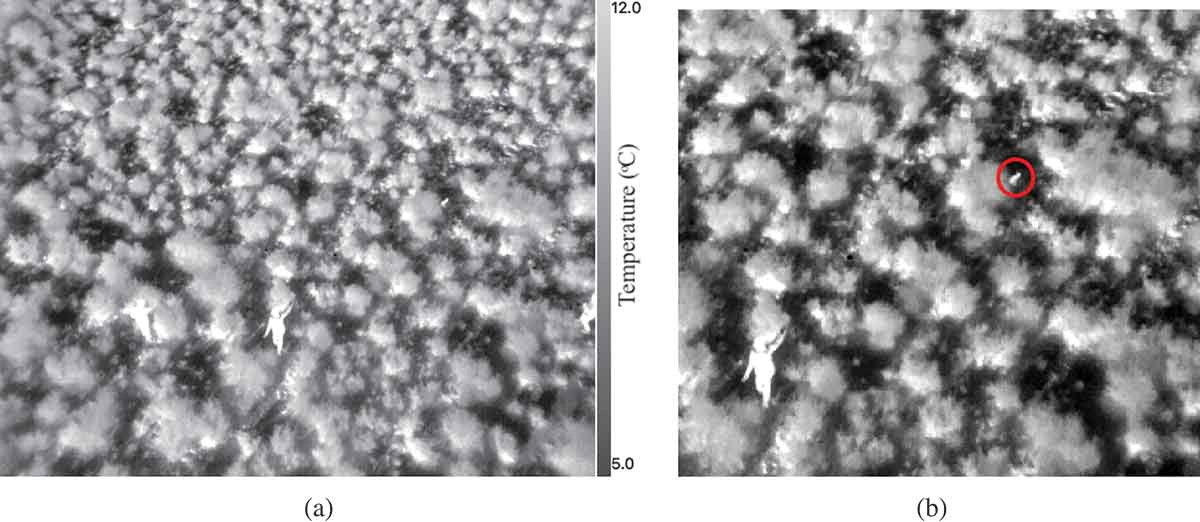
\includegraphics[scale=0.35]{images/tres_a_1558372_f0011_c.jpeg}
\caption{Detection of rabbit on field using thermal camera}\cite{animals_drone}
\label{fig:5}
\end{center}
\end{figure}

\section{Swarm flight path mapping}
\label{sec:3}
Despite all benefits, that drones bring to agriculture 4.0, it may be difficult for a single UAV to scan all required fields because of battery life limitations. It is possible that a coordinated effort of multiple drones can further reduce the time and energy required to sample data from each sensor in the field. For these reasons, flight path optimization models are currently in development for single-drone and multi-drone swarms to investigate their trade-offs. Agent-based models are usually developed, with the ability to generate flight paths for each drone within a swarm to scan all sensors within a simulated agriculture field (see Fig.~\ref{fig:6}). The simulations determine each drone’s aerial route for optimal flight path planning.
\cite{GOODRICH2023107591,agricultureswarm}

\begin{figure}[h]
\begin{center}
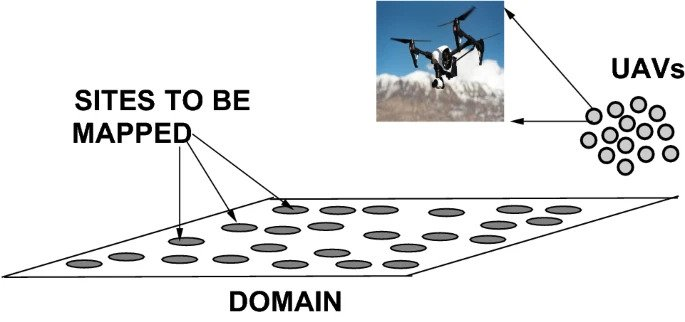
\includegraphics[scale=0.35]{images/ezgif.com-webp-to-jpg.jpg}
\caption{Example of problematics solved by swarm mapping}\cite{agricultureswarm}
\label{fig:6}
\end{center}
\end{figure}

The swarm modeling has origins in the description of biological groups (flocks of birds, schools of fish, crowds of human beings, etc.) responses to predators or prey. The system has many parameters, warranting the use of a Machine-Learning Algorithm. For example, UAVs equipped with cameras can collect videos or images for pre-emptive strategic analysis. Since the swarm would include UAVs to enable visible inspection with the cameras, one can implement a deep learning approach for image/video pattern/feature recognition. \cite{GOODRICH2023107591,agricultureswarm}


\newpage
\section{Conclusion}
\label{sec:4}
Drone technology is constantly evolving to meet agricultural needs. Agriculture is still in its early days, and it is likely that we will see even more benefits as technology develops. 
Farming drones can be one way to help reduce risk in several agribusinesses. Currently, there are UAVs that can provide real-time data to operators. This makes the economic advantages of drones more attainable. From lowering production costs to maximizing farming coverage, there really is no reason one shouldn’t make the switch. Drones were created to help people overcome obstacles in farming. This makes them an integral part of the human population’s ability to thrive through sustainable food production. The future is here, and it’s in the form of these farming drones. Success is within reach for those willing to adapt to it.

\newpage
% References

\begingroup
\makeatletter
\renewcommand\section{\@startsection {section}{1}{\z@}%
                                   {-3.5ex \@plus -1ex \@minus -.2ex}%
                                   {4.5ex \@plus.2ex}%
                                   {\large\bfseries}}
\makeatother


\bibliography{references}
\bibliographystyle{acm}
\endgroup

\end{document}


% ~\eqref{eq:01},~\eqref{eq:02},$\ldots$, (99).
% \begin{equation}z^{EO}=\min\limits_{e,\,g(\xi)}\mathbb{E}(F(\xi,e,g(\xi))),
% \label{eq:01}
% \end{equation}
% \begin{equation} a_{min}\leq a\leq a_{max}.
% \label{eq:02}
% \end{equation}


% \begin{theorem}
% This is a theorem content. Theorem text goes here. 
% \end{theorem}

% \begin{proof}
% Let $z$ be some element of $xH \cap yH$.  Then $z = xa$
% for some $a \in H$, and $z = yb$ for some $b \in H$.
% If $h$ is any element of $H$ then $ah \in H$ and
% $a^{-1}h \in H$, since $H$ is a subgroup of $G$.
% However, $zh = x(ah)$ and $xh = z(a^{-1}h)$ for all $h \in H$.
% Therefore $zH \subset xH$ and $xH \subset zH$, and thus
% $xH = zH$.  Similarly $yH = zH$, and thus $xH = yH$,
% as required.
% \end{proof}


% %
% % For figures use (also *.eps, *.tiff)
% %
% \begin{figure}[h]
% \begin{center}
% \includegraphics[scale=0.25]{images/i4c.png}
% \caption{Please write your figure caption here}
% \label{fig:1}
% \end{center}
% \end{figure}


% %
% % For tables use
% %
% \begin{table}[h] 
% \begin{center}
% \caption{Please write your table caption here} 
% \label{tab:1}
% \begin{tabular}{lll}
% \hline\noalign{\smallskip}
% Parameter & Symbol & Value\\
% \noalign{\smallskip}
% \hline\noalign{\smallskip}
% Param no. 1 & $\delta$ & 0\\
% Param no. 2 & $\pi$    & 3.14\\
% \hline
% \end{tabular}
% \end{center}
% \end{table}

% \section{Conclusion}
% \label{sec:2}
% \blindtext


% \begin{definition}
% Let $H$ be a subgroup of a group~$G$.  A \emph{left coset}
% of $H$ in $G$ is a subset of $G$ that is of the form $xH$,
% where $x \in G$ and $xH = \{ xh : h \in H \}$.
% Similarly a \emph{right coset} of $H$ in $G$ is a subset
% of $G$ that is of the form $Hx$, where
% $Hx = \{ hx : h \in H \}$
% \end{definition}